%-----------------------------------------------%
% Plano de Aula 01
%-----------------------------------------------%
\begin{anexosenv}     
    % \chapter{Acompanhamento de Aulas}
    % \begin{landscape}    
    % \end{landscape}
    % \chapter{Cronograma de aulas}
    % 	\includepdf[pages=-]{03-pos-textual/cronograma.pdf}
    \chapter{Materiais da Turma}
    \thispagestyle{empty}
    \label{anx:materiaisAnexo}
    
    \section{Unidade: Dilatação Térmica}
    \label{anx:materialAnexoDilatacaoTermica}
    Material de apoio desenvolvido pelo professor supervisor, para suporte às aulas de Dilatação Térmica. Este material encontra-se disponível para a turma no ambiente de ensino virtual \emph{Google Classroom} destacado pelo retângulo em vermelho na \autoref{fig:gClassroom}
    \vspace{1cm}
    \begin{figure}[!h]
        \centering
        \footnotesize        
        \caption{Print Screen do Google Classroom da Turma 2(5)}
        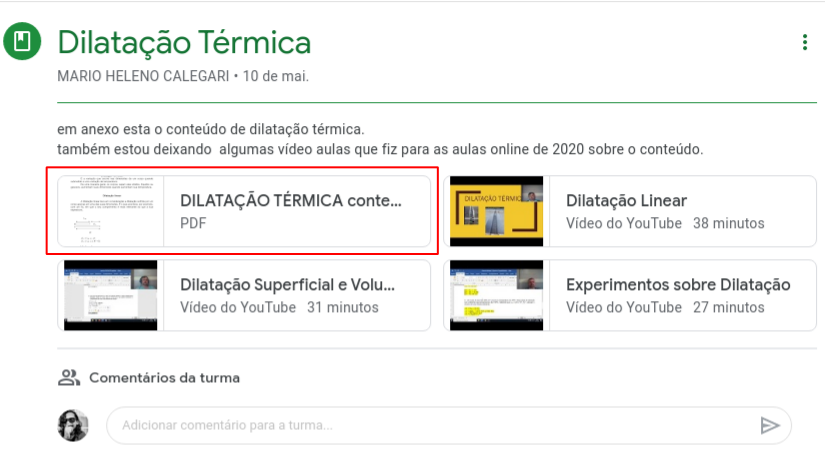
\includegraphics[width=\textwidth]{03-elementos/03.2_textual/03.2.1_fig/google-class01.png}
        \label{fig:gClassroom}
    \end{figure}

    Segue na integra:
    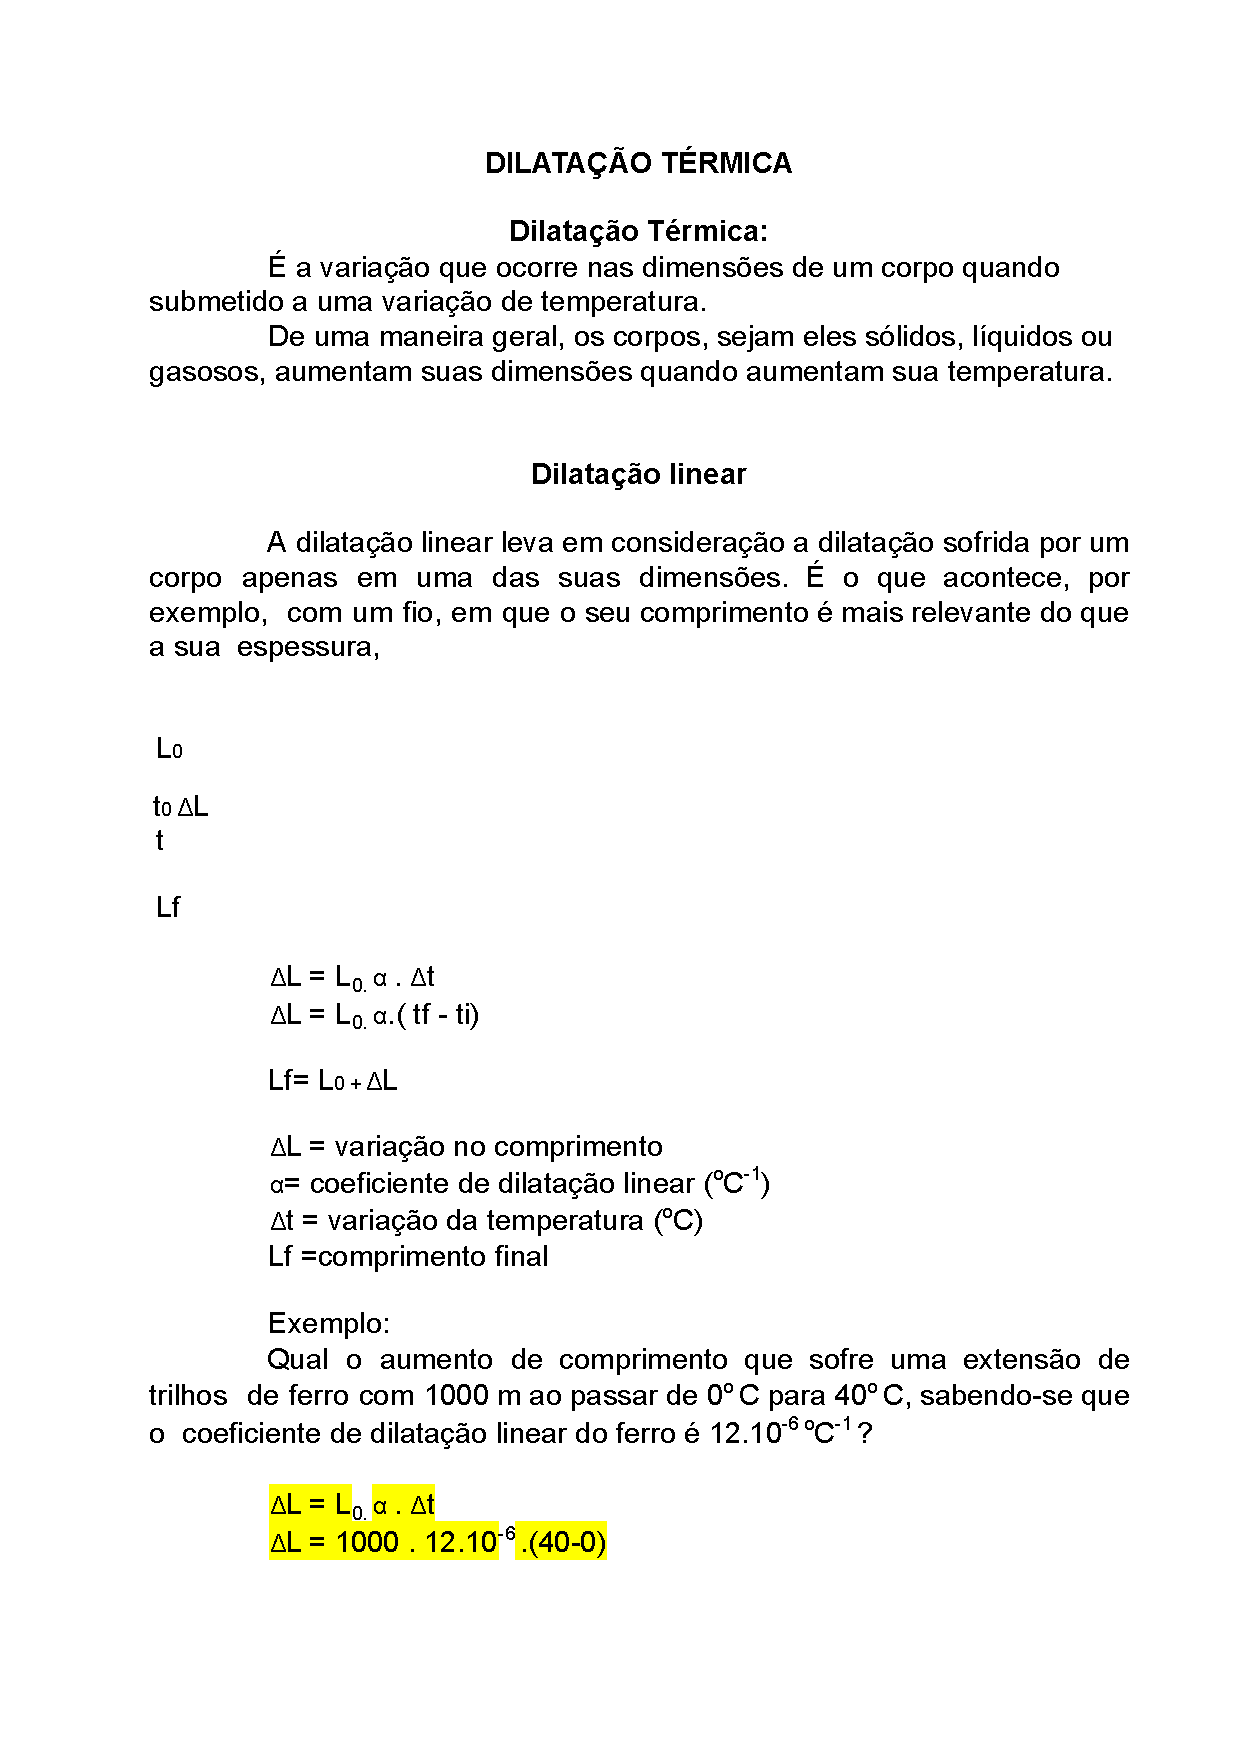
\includepdf[pages=-,scale=1]{03-elementos/03.2_textual/03.2.1_fig/apendice-I}
    % \includecode[shell]{l_olamundo}{Olá mundo em shell script}{03-elementos/03.2_textual/03.2.0_codes/ola.sh}

    % ROTEIROS EXPERIMENTAIS
    \chapter{Roteiros Experimentais}
    \label{anx:roteiros-experimentais}
    \section{Invisibilidade Observada Devido à Refração}
    \label{anx:invisibilidade-refracao}
    \subsection*{Materiais:}
    \begin{itemize}
        \item 1 béquer com $250\,\mathrm{ml}$ de água;
        \item 1 béquer com $250\,\mathrm{ml}$ de glicerina;
        \item 2 béquer de capacidade $50\,\mathrm{ml}$ vazio;
        \item 1 béquer com $500\,\mathrm{ml}$ de óleo de soja;
        \item 2 tubos de ensaio;
        \item 2 bastões de vidro;
        \item 1 pinça.
    \end{itemize}
    \subsection*{Procedimento:}
    \begin{enumerate}
        \item Introduzir o bastão de vidro primeiro na água e depois na glicerina e observar;
        \item Preencher um tubo de ensaio com óleo e inserir no béquer de $500\,\mathrm{ml}$ de óleo;
        \item No mesmo béquer de $500\,\mathrm{ml}$ de óleo, inserir outro tubo de ensaio vazio e comparar com o tubo de ensaio que está cheio de óleo;
        \item No tubo de ensaio vazio, que está dentro do béquer com óleo, colocar água lentamente até a metade do tubo e observar;
        \item Ainda no tubo de ensaio contendo água, preencher lentamente com óleo e observar. 
    \end{enumerate}
    \subsection*{Questões:}
    \begin{quest}
        Por que o bastão de vidro "desaparece" quando colocamos na glicerina?
    \end{quest}
    \begin{quest}
        Como explicar o fato do tubo de ensaio desaparecer quando inserimos óleo?
    \end{quest}
\end{anexosenv}